\section{Reeb graphs as Metric Measure Spaces}\label{sec:reeb_mms}

In this article, we aim at comparing Reeb graphs and Mapper graphs using tools and distances for metric spaces. In this section, we first define a metric structure on the Reeb graph using the Hausdorff distance, and then we study the induced topology of this corresponding metric space.

\subsection{Hausdorff distance on Reeb graphs}

We will denote the set of non-empty compact subsets of a metric space $(\spa,\dis)$ as $\comp(\spa)$.  See~\cite{henrikson1999completeness} for a comprehensive introduction of the Hausdorff distance. 

\begin{definition}{Hausdorff distance.}\\
 Let $A,B$ be two subsets of a metric space $(\spa,\dis)$, the Hausdorff distance between $A$ and $B$ is defined as:
 $$\haus(A,B)=\max\left(\sup_{x\in A}\dis(x,B),\sup_{y\in B}\dis(y,A)\right),$$
 where $\dis(x,B)=\inf_{v\in B}\dis(x,v)$ and $\dis(y,A)=\inf_{u\in A}\dis(u,y)$.
\end{definition}
%Note that for arbitrary subsets $A$ and $B$, $\haus$ can be $+\infty$.
With the same notations as before,  
the Hausdorff distance
can be equivalently defined as:
$$\haus(A,B)=\inf\left\{\eps>0,\,A\subseteq B^\eps\;\mathrm{ and }\;B\subseteq A^\eps\right\},$$
where $C^\eps=\bigcup_{z\in C}\ball(z,\eps)$ for every subset $C$ of $X$.

%Let us recall two basic properties of the Hausdorff distance,. With the same notations as before and denoting for every subset $C$ of $X$: $C^\epsilon=\bigcup_{z\in C}\ball_\epsilon(z).$
%\begin{proposition}
%The Hausdorff distance
%can be equivalently defined as:
%$\haus(A,B)=\inf\left\{\epsilon>0,\,A\subseteq B^\epsilon\;\mathrm{ and }\;B\subseteq A^\epsilon\right\}.$
%\end{proposition}
The Hausdorff distance 
$\haus$ is a metric on $\comp(\spa)$. Moreover, the topology of $(\comp(\spa),\haus)$ follows closely from the topology of $(\spa,\dis)$. We illustrate this with the two following propositions proved in~\cite{henrikson1999completeness}.

\begin{proposition}\label{prop:haus_limit}
Suppose that $(\spa,\dis)$ is complete. Then $(\comp(\spa),\haus)$ is also complete. Moreover, let $(a_n)_{n\in\N}$ be a Cauchy sequence in $(\comp(\spa),\haus)$, then $a_n\converge a$, where:
$$a=\left\{x \in \spa, \, \textrm{ there exists a sequence } (x_n)_{n\in\N}  \in \prod_n a_n  \textrm{ such that } x_n \converge x \right\}.$$
\end{proposition}

\begin{proposition}
If $(\spa,\dis)$ is compact then $(\comp(\spa),\haus)$ is also compact.
\end{proposition}

Hereafter, $(\man,\dis)$ is assumed to be a connected compact Riemannian manifold together with its geodesic distance. We also consider a Morse function $f\colon\man\rightarrow\R$. 
%Like mentioned before, %in Proposition~\ref{prop:morse}, 
%choosing $f$ to be Morse is a fairly generic choice.
In this section, to alleviate notations, we will denote the Reeb graph $\Reeb_f(\man):=\man/\sim_{f}$ by $\reeb$.

In order to use the Hausdorff distance, we prove the following:

\begin{proposition}\label{prop:reeb_closed}For every $a\in\reeb$, $a$ is closed as a subset of $\man$.
\end{proposition}
\begin{proof}
Let $a\in\reeb$, then $a$ is defined as a connected component of $\preim{f}{\{v\}}$ for some $v$ in $f(\man)$. The set
$a$ is therefore closed in $\preim{f}{\{v\}}$ since it is a connected component, as connected components are maximal connected subsets and the closure of a connected subset is also connected. Moreover, $\preim{f}{\{v\}}$ is closed in $\man$ because $f$ is continuous. As such, $a$ is closed in a closed subset and consequently closed in $\man$.
\end{proof}

The manifold $\man$ being compact, Proposition~\ref{prop:reeb_closed} proves that $\reeb\subseteq\comp(\man)$. Thus, $(\reeb,\haus)$ is a metric space.

\subsection{Topology of \texorpdfstring{$(\reeb,\haus)$}{TEXT}}
In order to define Wasserstein and Gromov-Wasserstein distances on top of $(\reeb,\haus)$, the space $\reeb$ needs to be complete and separable. However, we first show that this metric space is not complete in general (see Figure \ref{fig:reeb_adherence}). To circumvent this, we consider its closure $\overline{\reeb}$, which is compact and as such complete. We show that $\reeb$ differs from $\overline{\reeb}$ only by a finite number of points. 
%Accordingly, we will work afterwards in the complete and separable metric space $(\overline{\reeb},\haus)$.\\
Let us start with preliminary results.

\begin{proposition}\label{prop:reeb_adherence} Let $a\in\comp(\man)$ be an adherent point to $\reeb$. Then $a$ is connected and $f$ is constant on $a$.

\end{proposition}
\begin{proof}
Let $a\in\comp(\man)$ such that there exists $(a_n)_{n\in\N}\in\left(\reeb\right)^{\N}$ that converges to $a$.

$\bullet$ We first show that $a$ is connected. 
    Suppose that $a$ is not connected. Since it is compact, this means that it can be written as the disjoint union of two compact sets $a_0\sqcup a_1$.  Now, $a_0$ and $a_1$ being disjoint and both compact, there exists $\eps>0$ such that $a_0^\eps$ and $a_1^\eps$ are disjoint. To see this, consider for example $\eps :=\frac{1}{2}\ \inf_{x\in a_0,y\in a_1}\dis(x,y)$  and notice that $\inf_{x\in a_0,y\in a_1}\dis(x,y)>0$ by compactness of $a_0$ and $a_1$. \\
    Next, there exists a rank $N\in\N$ such that $\haus(a_N,a)\leq\frac{\eps}{2}$. This means that 
     $a_N\subseteq a^{\frac{\eps}{2}}=a_0^{\frac{\eps}{2}}\sqcup a_1^{\frac{\eps}{2}},$ 
    and since $a_N$ is connected, it is included in one of $a_0^{\frac{\eps}{2}}$ and $a_1^{\frac{\eps}{2}}$ and not in the other. W.l.o.g.,
    %By symmetry, 
    we suppose that it is included in $a_0^{\frac{\eps}{2}}$. 
    Let $x\in a_1$, there exists $z\in a_N$ such that $\dis(x,z)\leq\frac{\eps}{2}$ because $a\subseteq a_N^{\frac{\eps}{2}}$. 
    In the same way, there exists $y\in a_1$ that satisfies $\dis(y,z)\leq\frac{\eps}{2}$, since $a_N\subseteq a_0^{\frac{\eps}{2}}$. 
    However, this means that there exist two points $(x,y)\in a_0\times a_1$ such that $\dis(x,y)\leq \eps$ and this contradicts the fact that $a_0^\eps$ and $a_1^\eps$ are disjoint. Note that we have shown more generally that every limit in the Hausdorff distance  of a sequence of connected compact sets is connected.
    
    
    
$\bullet$ We now show that $f$ is constant on $a$. 
    Let $x,y\in a$. By Proposition~\ref{prop:haus_limit}, we know that there exist two sequences $(x_n)_{n\in\N}$ and $(y_n)_{n\in\N}$ in $(a_n)_{n\in\N}$ such that $x_n\converge x$ and $y_n\converge y$. 
    Now, for every $n$, since  $x_n,y_n\in a_n$, then $f(x_n)=f(y_n)$ as $f$ is constant on $a_n$. Using this fact, we have:
    \begin{align*}
        | f(x)-f(y) |&\leq | f(x)-f(x_n) | + | f(x_n)-f(y_n) |+ | f(y_n)-f(y) |\\
        &\leq | f(x)-f(x_n) | + | f(y_n)-f(y) |.
    \end{align*}
    By continuity of $f$, it yields that $f(x)=f(y)$.
 

\end{proof}

The second point of Proposition~\ref{prop:reeb_adherence} proves that we can define a function $\Tilde{f}\colon \overline{\reeb}\rightarrow\R$ that associates to every adherent point of $\reeb$ the constant value that $f$ takes on it. Proposition~\ref{prop:reeb_adherence} as a whole might seem to indicate that $\overline{\reeb}=\reeb$ could also be proved, %with a bit more of work, 
but this turns out to be false in general. The crucial property that the elements of $\overline{\reeb}\setminus\reeb$ do not satisfy %lack to be in $\reeb$ 
is to be associated to {\it maximal} connected subsets. See Figure \ref{fig:reeb_adherence} for an example.
However, we now prove that $\overline{\reeb}$ and $\reeb$ differ only by a finite number of points.

\begin{figure}[t]
    \centering
    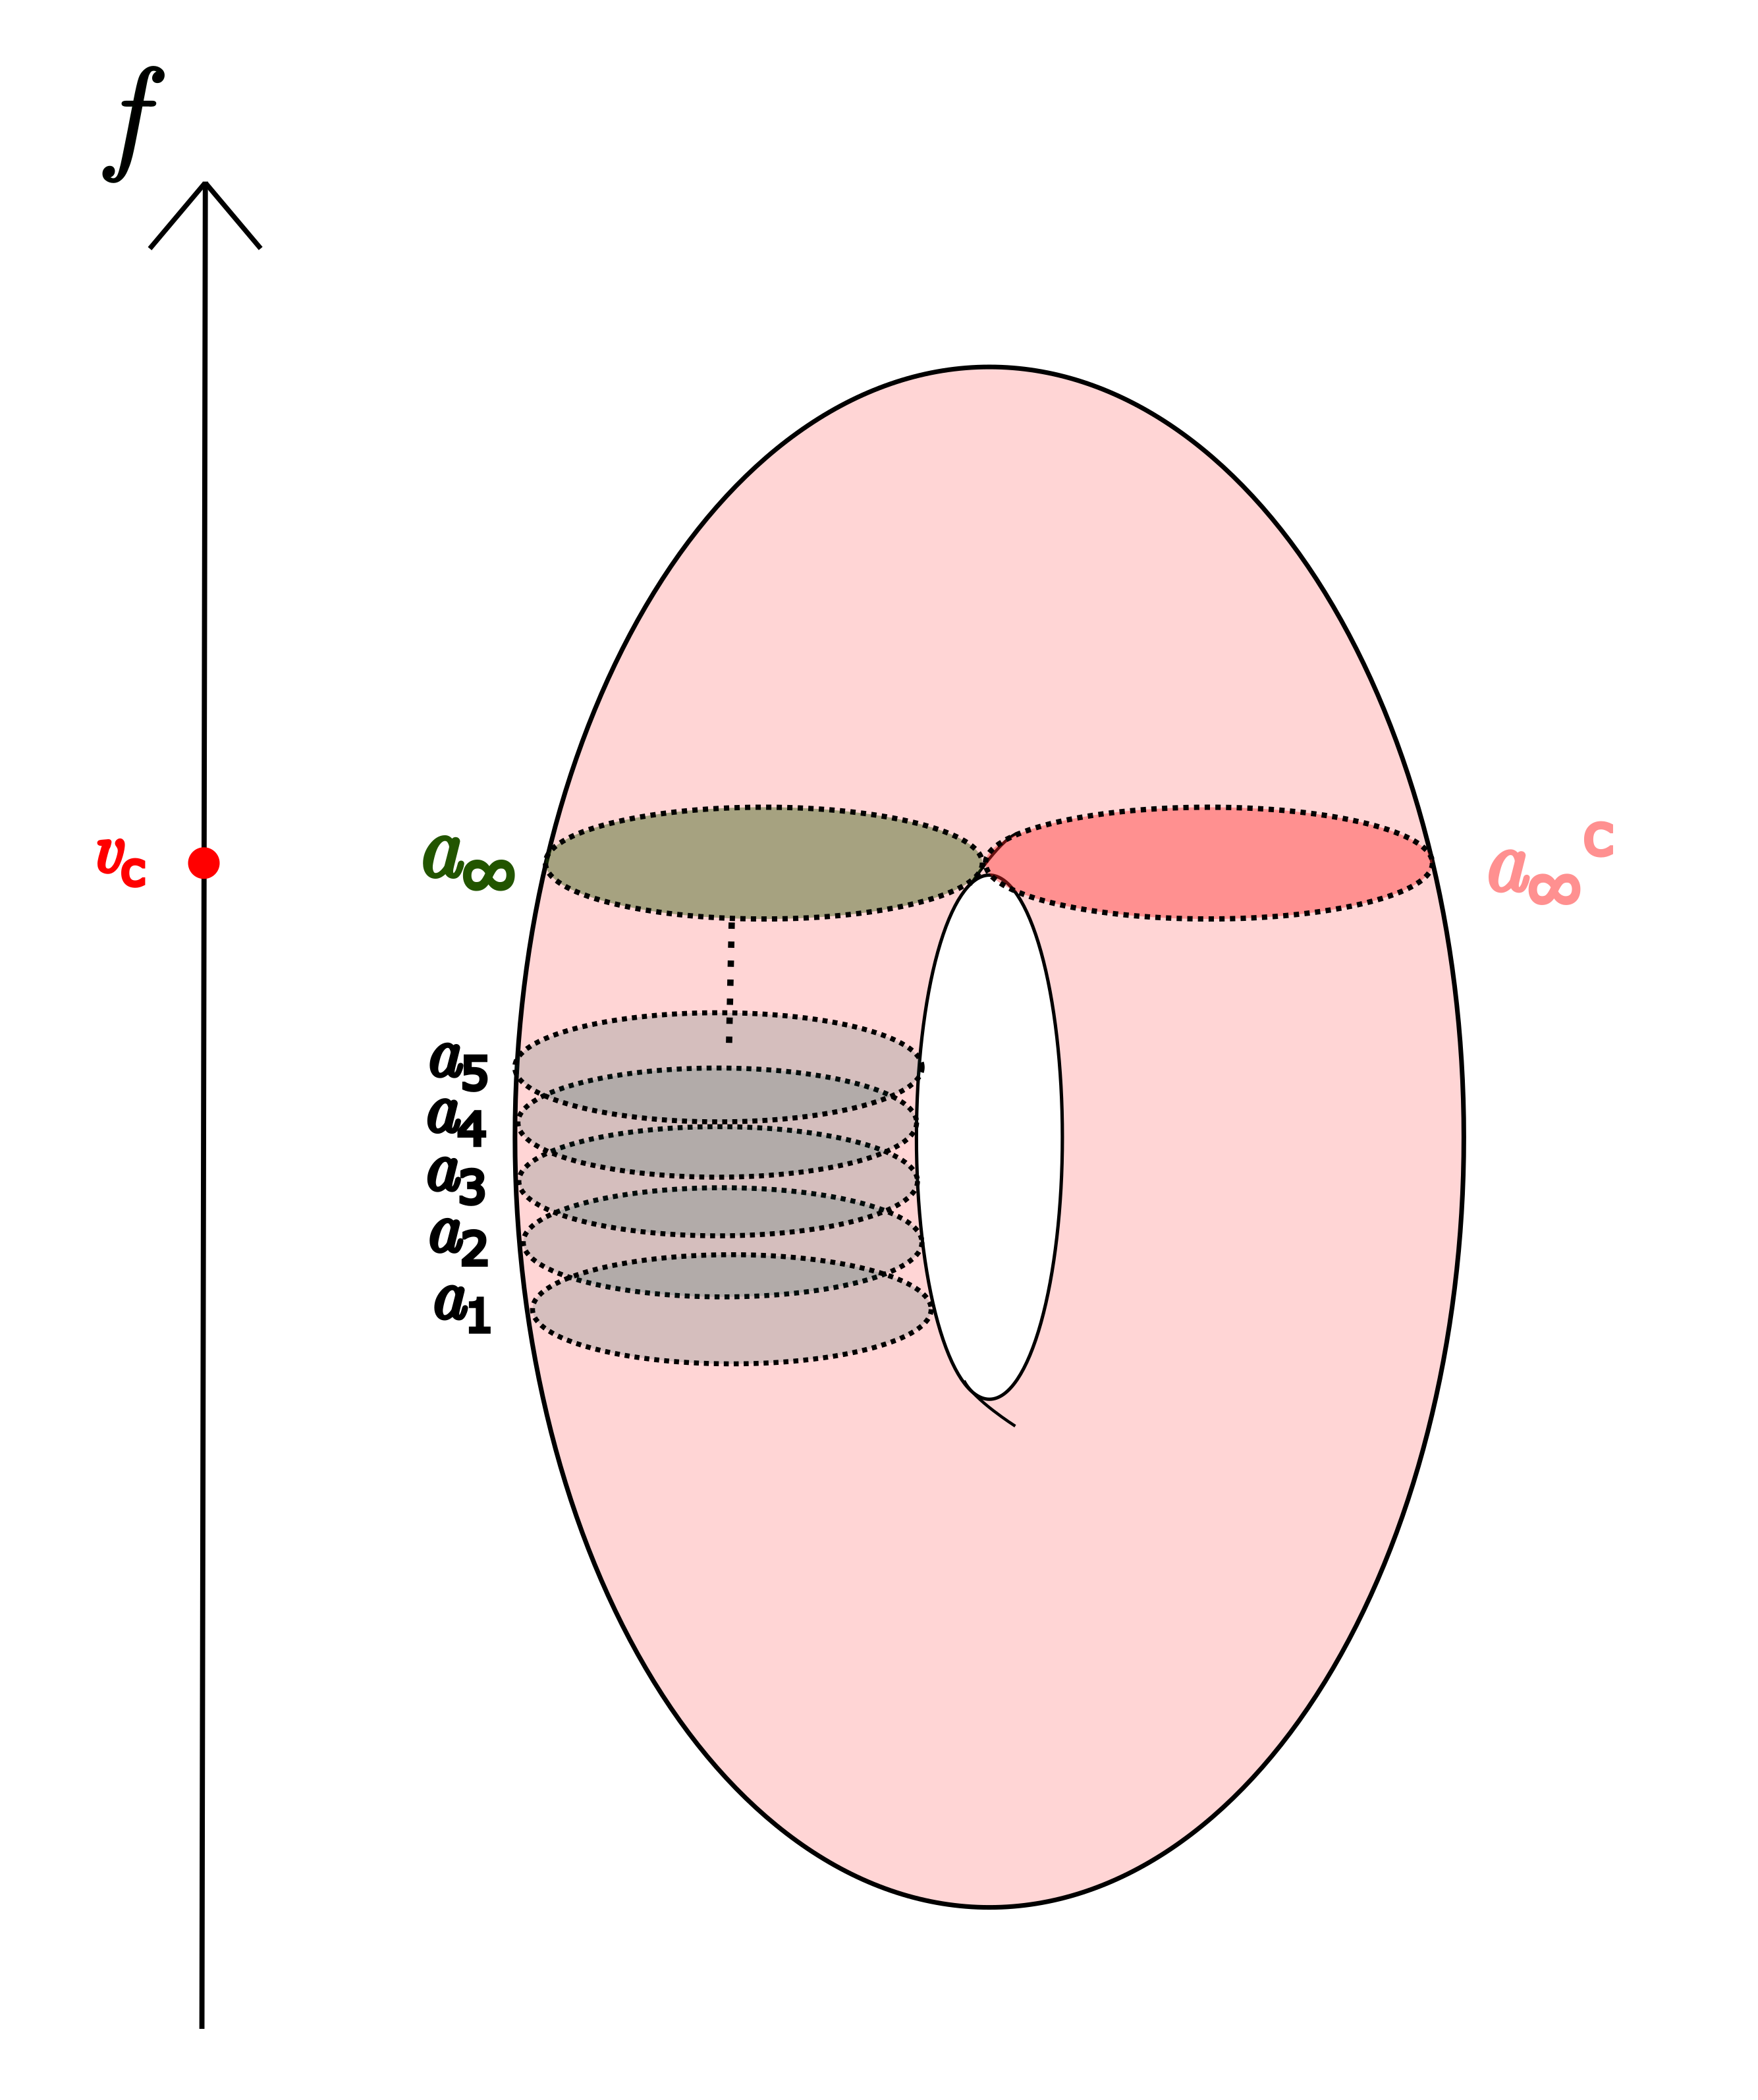
\includegraphics[width=0.4\textwidth]{images/reeb_adherence.png}
    \caption{Example of a Reeb graph sequence $(a_n)_{n\in\N}$ that has a Hausdorff limit $a_\infty$ outside of the Reeb graph. Notice that this occurs when $a_\infty$ is inside the level set of a critical value $v_c$. In this example, $\preim{f}{\{v_c\}}$ has only one connected component. The complement $a_\infty^c$ of $a_\infty$ in this connected component is also represented here.}
    \label{fig:reeb_adherence}
\end{figure}

\begin{lemma}\label{lem:haus_cont}
Let $(a_n)_{n\in\N}\in\reeb^{\N}$ and $(x_n)_{n\in\N}\in\man^{\N}$, such that $x_n\in a_n$ 
%(equivalently $a_n=[x_n]_{\sim_f}$) 
for every $n\in\N$ and such that $(x_n)_{n\in\N}$ admits a limit $x \in \man$. 
If $f(x)$ is not a critical value, then $a_n\converge [x]_{\sim_f}$.
\end{lemma}
\begin{proof}
Let $(a_n=[x_n]_{\sim_f})_{n\in\N} \in \reeb^{\N}$ be such that $(x_n)_{n\in\N}$ admits a limit $x \in \man$. As $\overline{\reeb}$ is compact, it converges if and only if it has one and only one adherent point. It admits an adherent point by compactness of $\overline{\reeb}$ and we have to show that it is unique and equal to $[x]_{\sim_f}$. Let $(a_{\phi(n)})_{n\in\N}$ be a subsequence of $a_n$ that converges to an element $a\in\overline{\reeb}$. 

$\bullet$ We first show that $a\subseteq[x]_{\sim_f}$. By Proposition~\ref{prop:haus_limit}, we know that:
%$$a=\left\{y,\,\exists(y_n)_n:\,\left[y_n\converge y\text{ and }\forall n, y_n\in a_{\phi(n)}\right]\right\}.$$
$$a=\left\{y \in \man \, , \textrm{ there exists a sequence } (y_n)_n  \in \prod_n a_{\phi(n)} 
\textrm{ such that } y_n \converge y \right\}.$$
Now, $(x_{\phi(n)})_{n\in\N}$ is a subsequence of $(x_n)_{n\in\N}$ and as such $x_{\phi(n)}\converge x$. Therefore, $x\in a$, and furthermore by Proposition~\ref{prop:reeb_adherence}, $a$ is connected and included in $\preim{f}{\{v\}}$, where $v=f(x)$. These three points prove that $a\subseteq[x]_{\sim_f}$, since by definition $[x]_{\sim_f}$ is the maximal subset that verifies these three exact requirements. 

$\bullet$ We now show that $[x]_{\sim_f}\subseteq a$. Let $y\in[x]_{\sim_f}$. As $v=f(x)$ is not a critical value, by Theorem~\ref{thm:morse}, there exists $\eps>0$ and a homeomorphism $\psi:\preim{f}{\{v\}}\times[-\eps,\eps] \rightarrow \preim{f}{[v-\eps,v+\eps]}$. 
Since $f$ is continuous, there exists a rank $N\in\N$ such that $\forall n\geq N$: $|f(x_{\phi(n)})-v|\leq \eps$. Therefore, the following sequence is well defined:
$$\forall n\in\mathbb{N}:\,y_n=\begin{cases}
    x_{\phi(n)}&\text{ if } n<N,\\
    \psi\left(y,f(x_{\phi(n)})-v\right)&\text{otherwise}.
\end{cases}$$
By continuity of $\psi$ and $f$, $y_n\converge y$ (since $\psi(\cdot,0)$ is the identity by construction of $\psi$, see the proofs of Lemma~\ref{lem:flow} and Theorem~\ref{thm:morse}). It only remains to show that for a large enough rank $M\in\N$, one has $y_n\in a_{\phi(n)}$,
%for every $n\geq M$, 
to conclude that $y\in a$.\\\\
On one hand, since $v$ is not a critical value, $\preim{f}{\{v\}}$ is a submanifold of $\man$ by the Implicit Function Theorem (see Theorem 5.8. of~\cite{boothby1986introduction} for example). The set $\preim{f}{\{v\}}$ is hence locally path-connected. Thus, there exists $\delta>0$ such that for all  $z\in \preim{f}{\{v\}}$, $\dis(x,z)\leq\delta$ implies that $z\in[x]_{\sim_f}$.\\\\
On the other hand, by continuity, we have $\preim{\psi}{x_{\phi(n)}}\converge \preim{\psi}{x}=(x,0)$. From the expression of $\psi^{-1}$ given in the proof of Theorem~\ref{thm:morse}, we find that   $\preim{\psi}{x_{\phi(n)}}=\left(z_n,w_n\right)$ where $z_n \in \preim{f}{\{v\}}$ and  $w_n=f(x_{\phi(n)})-v$. Thus, there exists a rank $M\in\N$ such that $\forall n\geq M$: $\dis(z_n,x)\leq\delta$ and then 
 $z_n$ and $y$ are in the same connected set $[x]_{\sim_f}$. Moreover, by continuity of the map $\psi\left(\cdot,w_n\right) : \preim{f}{\{v\}} \rightarrow  \preim{f}{\{w_n\}}$, the images  $x_{\phi(n)} = \psi\left(z_n,w_n\right)$ and $y_n = \psi\left(y,w_n\right)$  are carried to the same connected component of $\preim{f}{\{w_n\}}$. Consequently $y_n\in[x_{\phi(n)}]_{\sim_f}$ and we know that $[x_{\phi(n)}]_{\sim_f}=a_{\phi(n)}$. See Figure \ref{fig:lemma_continuity} for an illustration.

Finally, $(a_n)_{n\in\N}$ admits one and only one adherent point, which is $[x]_{\sim_f}$.

\begin{figure}[t]
    \centering
    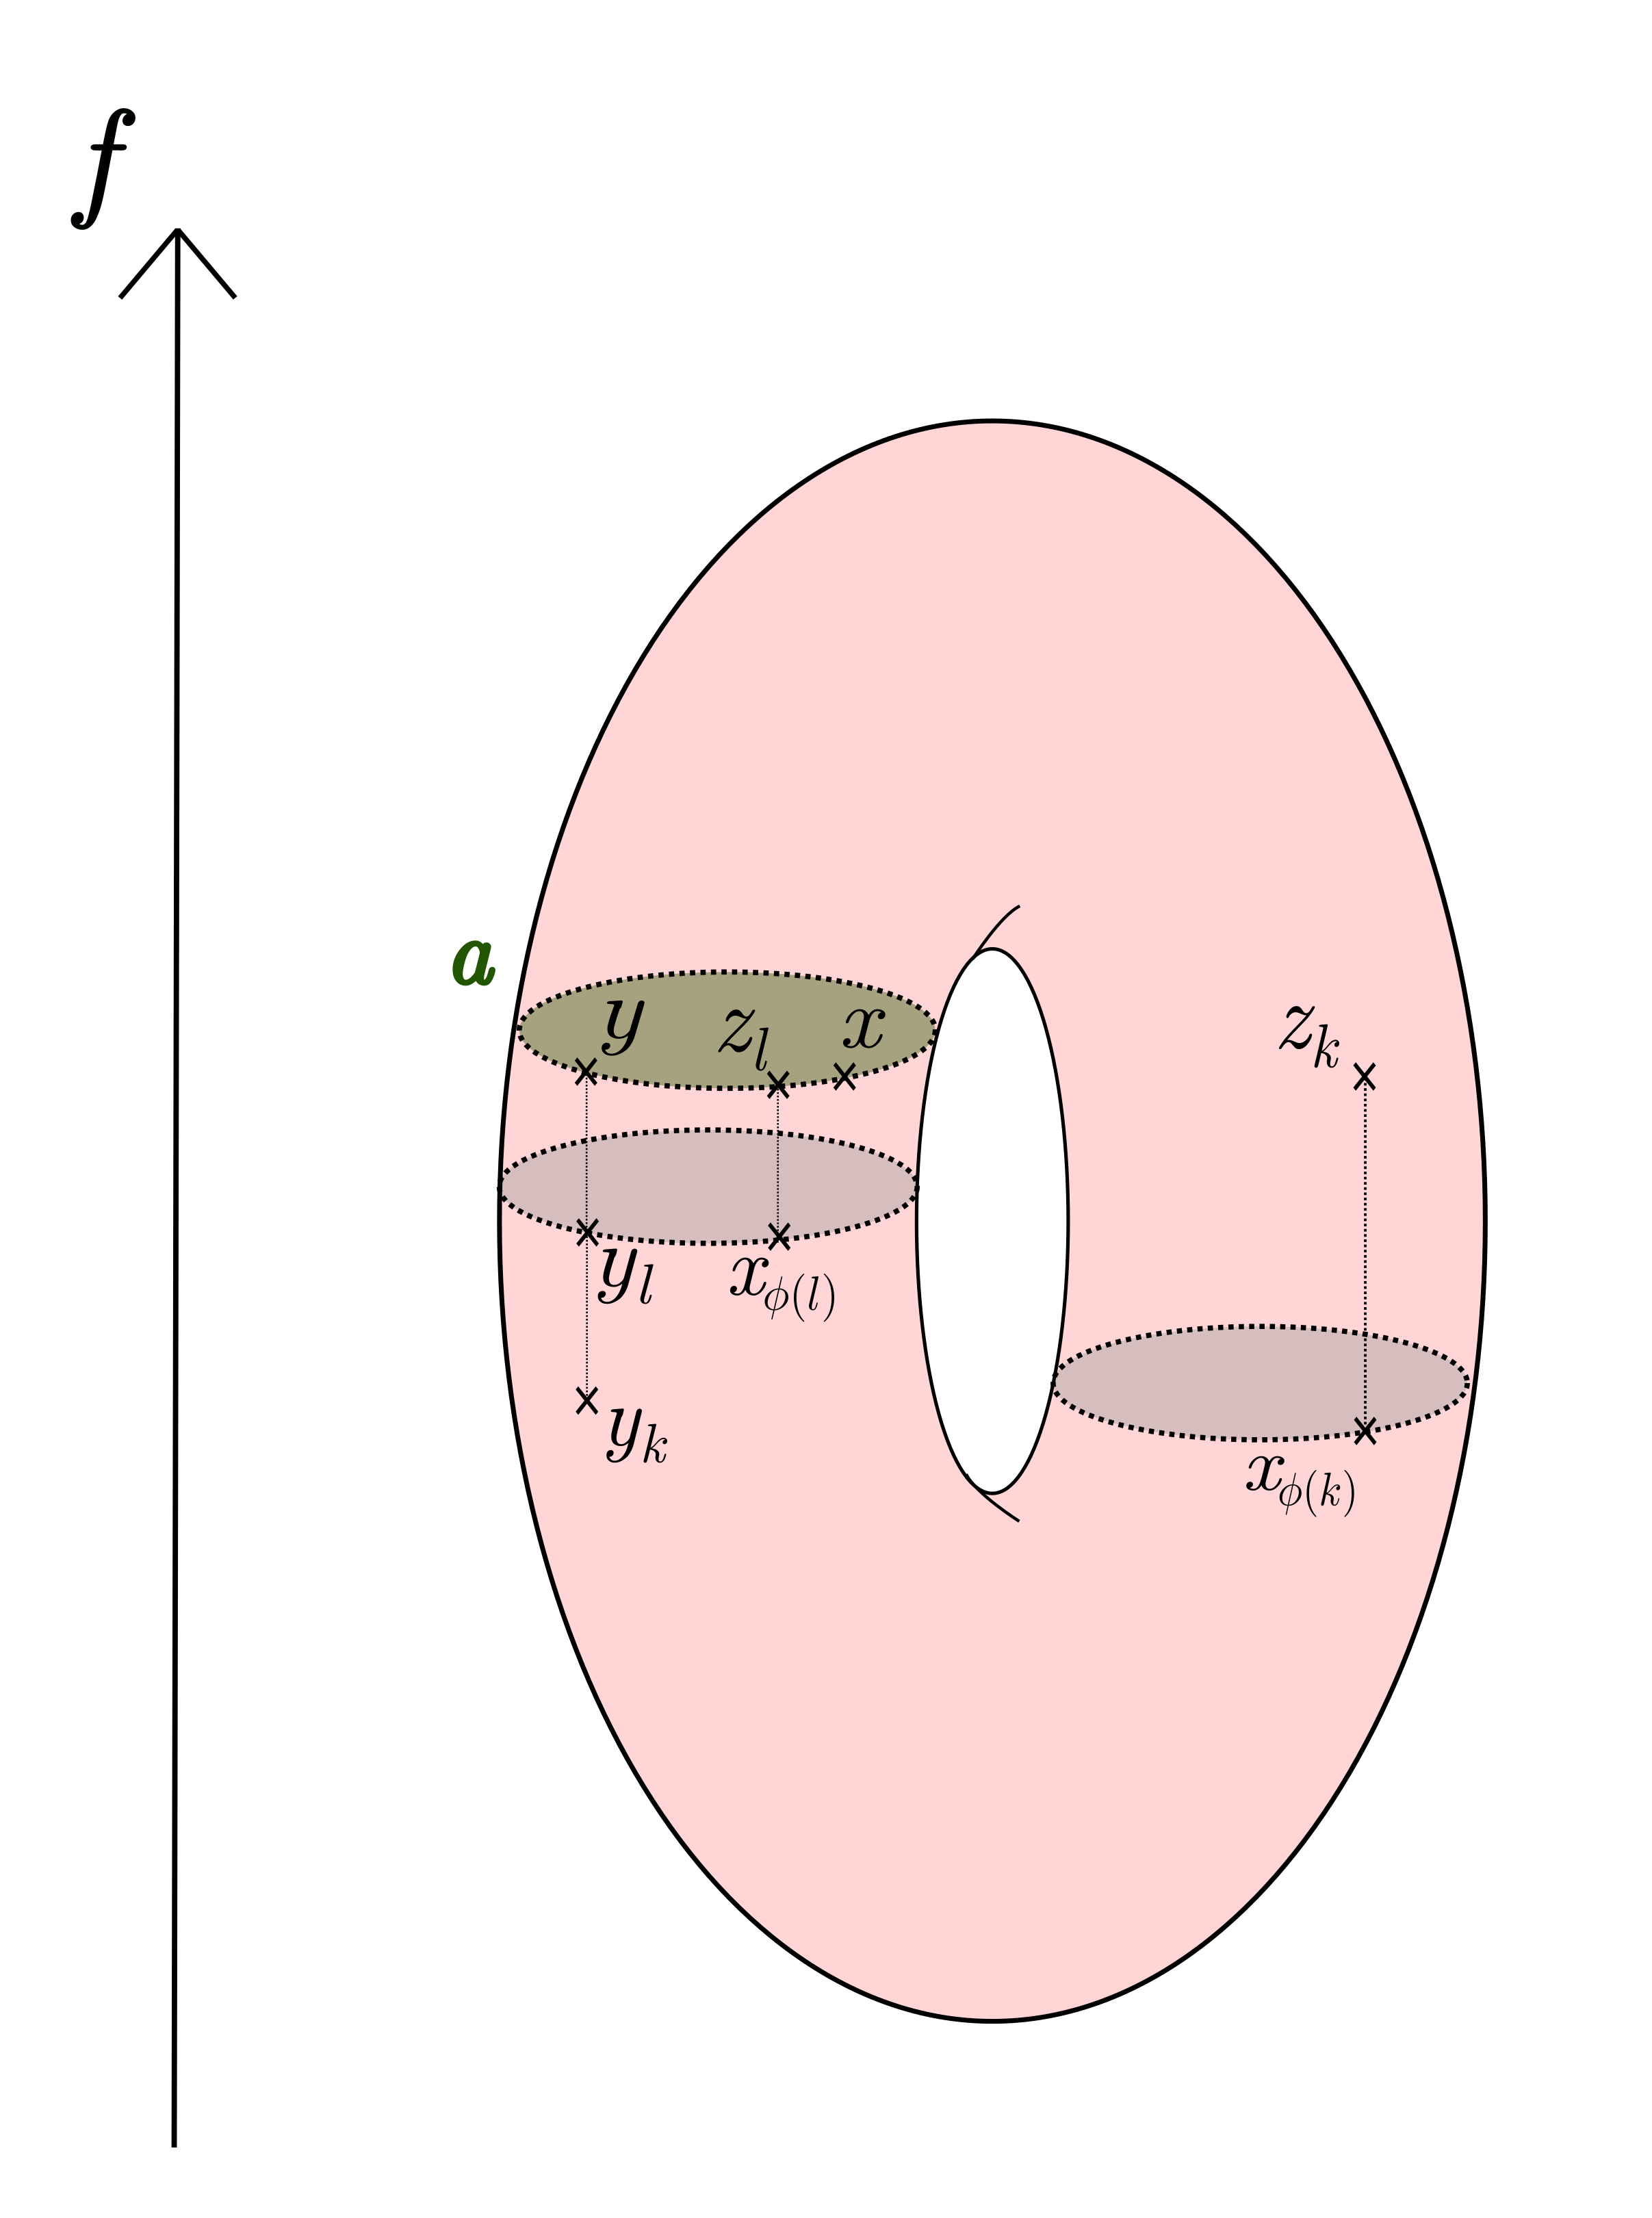
\includegraphics[width=0.4\textwidth]{images/lemma_continuity.png}
    \caption{Illustration of the argument made in the proof of Lemma \ref{lem:haus_cont}. Two points $x_{\phi(k)}$ and $x_{\phi(l)}$ of the sequence $(x_{\phi(n)})_{n\in\N}$ are given as examples. The sequence $(z_n)_{n\in\N}$ is made of the projections of the elements of $(x_{\phi(n)})_{n\in\N}$ onto the level set where $a$ belongs using the gradient flow. Similarly, the sequence $(y_n)_{n\in\N}$ is made of the projections of $y$ onto the level sets $\preim{f}{\{x_{\phi(n)}\}}$. We see that, by continuity, $(z_n)_{n\in\N}$ must be in $a$ (for a large enough rank). This means that after this rank, $y_n$ and $x_{\phi(n)}$ must be in the same element of the Reeb graph.}
    \label{fig:lemma_continuity}
\end{figure}

\end{proof}

\begin{proposition}\label{prop:reeb_finite}
$\overline{\reeb}\setminus\reeb$ is finite.
\end{proposition}
\begin{proof}
Recall that $\Tilde{f}\colon \overline{\reeb}\rightarrow\R$ is defined as the function that associates any adherent point of $\reeb$ to the constant value that $f$ takes on it. Let $\psi_{\cdot}$ be the gradient flow of $f$.


 Let $a\in\overline{\reeb}$ be non-empty. First, assume that $v=\Tilde{f}(a)$ is not a critical value of $f$. Let $(a_n)_{n\in\N}$ be a sequence of elements in $\reeb$ that converges to $a$. Let $x\in a$ and choose a sequence $(x_n)_{n\in\N}$ such that $x_n\in a_n$ for every $n\in\N$ and $x_n\converge x$. By Lemma~\ref{lem:haus_cont}, $a_n\converge[x]_{\sim_f}$ and as such $a=[x]_{\sim_f}$ and in particular  $a\in\reeb$. We thus have showed that for any  $a\in\overline{\reeb}\setminus\reeb$ which is non empty, $\Tilde{f}(a)$ is a critical value.
 
We continue the proof of the proposition with the following lemma.

\begin{lemma} 
\label{lem:3cases}
Let $a\in\overline{\reeb}$ such that $v=\Tilde{f}(a)$ is a critical value. Let $v^-$ (resp. $v^+$) denote the closest critical value $v'$ to $v$ satisfying $v'<v$ (resp. $v'>v$) if it exists.  
Let also $(a_n)_{n\in\N}$ be a sequence of elements in $\reeb$ that converges to $a$. Then, we can extract a subsequence $(a_{\phi(n)})_{n\in\N}$ from $(a_n)_{n\in\N}$ such that one of the three following assertions is satisfied:
\begin{enumerate}
    \item $\forall n\in\mathbb{N}, $ $\Tilde{f}(a_{\phi(n)})=\Tilde{f}(a) = v$;
    \item there exists a connected component $c$ of $\preim{f}{\{\frac{v^-+v}{2}\}}$ such that $\forall n\in\N$, $a_{\phi(n)}=\psi_{v_n-(\frac{v^-+v}{2})}(c)$ where $v_n\in(\frac{v^-+v}{2},v) $, and $(v_n)_{n\in\N}$ converges to $v$;
    \item there exists a connected component $c$ of $\preim{f}{\{\frac{v+v^+}{2}\}}$  such that $\forall n\in\N$, $a_{\phi(n)}=\psi_{v_n-(\frac{v+v^+}{2})}(c)$ where $v_n\in(v,\frac{v+v^+}{2})$, and $(v_n)_{n\in\N}$ converges to $v$.
\end{enumerate}
\end{lemma}

\begin{proof}
If there exists a rank after which the sequence $(a_n)_{n\in\N}$ verifies $\Tilde{f}(a_n)=v$, then the first assertion is satisfied. In the following of the proof, we thus assume that $\forall n\in\N$, there exists $N_n\geq n$ such that $\Tilde{f}(a_{N_n})\neq v$. This allows us to extract a subsequence $(a_{\phi(n)})_{n\in\N}$ that satisfies $\Tilde{f}(a_{\phi(n)})\neq v$ for all $n\in\N$. W.l.o.g., by re-extracting, we can assume that $\forall n\in \N,\,\Tilde{f}(a_{\phi(n)})< v$.

%Moreover, either there exists a rank after which $\Tilde{f}(a_{\phi(n)})< v$, or by the same argument we can extract a further subsequence $(a_{\phi'(n)})_n$ that verifies $\Tilde{f}(a_{\phi'(n)})> v$.\\
%In summary, we are able to extract from $(a_n)_n$ a subsequence $(a_{\phi(n)})_n$ that either verifies
%\begin{itemize}
 %   \item $
%(\forall n\in \mathbb{N},\,\Tilde{f}(a_{\phi(n)})< v)$ or,
%\item $(\forall n\in \mathbb{N},\,\Tilde{f}(a_{\phi(n)})> v)$.
%\end{itemize}
%We continue by assuming the first case, the proof for the second is symmetrical.\\

Notice that $a_{\phi(n)}\converge a$. Let $x\in a$ and $(x_n)_{n\in\N}\in(a_{\phi(n)})_{n\in\N}$ such that $x_n\converge x$. 
By continuity of $f$, there exists $N\in\N$, such that $\forall n\geq N$, $f(x_n)\in(\frac{v^-+v}{2},v)$.
$[\frac{v^-+v}{2},f(x_n)]$ does not contain critical values. As such, we can construct a diffeomorphism $\psi_{f(x_n)-\frac{v^-+v}{2}}$ between $\preim{f}{\{\frac{v^-+v}{2}\}}$ and $\preim{f}{\{f(x_n)\}}$ using the gradient flow of $f$, see Lemma~\ref{lem:flow} for more details. 

Consider now the connected components $(c_i)_i$ of $\preim{f}{\{\frac{v^-+v}{2}\}}$. We will prove that: $$ \exists i,\,\forall n\in\N,\,\exists k_n\geq n:\,a_{\phi(k_n)}=\psi_{f(x_{k_n})}(c_i) .$$
The opposite of this means that for all connected components $c_i$ there is a rank $n_i$ such that $\forall k\geq n_i$: $a_{\phi(k)}$ is not diffeomorphic to $c_i$. Since the number of $(c_i)_i$ is finite (see Proposition~\ref{prop:local_path_con}), taking $K=\max_i n_i$, we would have that $\forall k\geq K$, $a_{\phi(k)}$ is not diffeomorphic to any of the $c_i$ under the flow $\psi_{f(x_k)-\frac{v^-+v}{2}}$. This contradicts that $\forall n\geq N$: $\preim{f}{\{f(x_n)\}}$ and $\preim{f}{\{\frac{v^-+v}{2}\}}$ are diffeomorphic under the flow $\psi_{f(x_k)-\frac{v^-+v}{2}}$, and that this diffeomorphism induces a bijection between connected components. This can be understood as a application of the pigeonhole principle, see Figure \ref{fig:reeb_tirroir} for an illustration. 

This allows to extract a further subsequence $(a_{\Phi(n)})_{n\in\N}$ that converges to $a$, and that consists only of diffeomorphic images of a fixed connected component $c_i$, under well determined maps $(\psi_{v_n-\frac{v^-+v}{2}})_{n\in\N}$ such that $v_n\converge v$.
 
We therefore proved the lemma.

\begin{figure}[t]
    \centering
    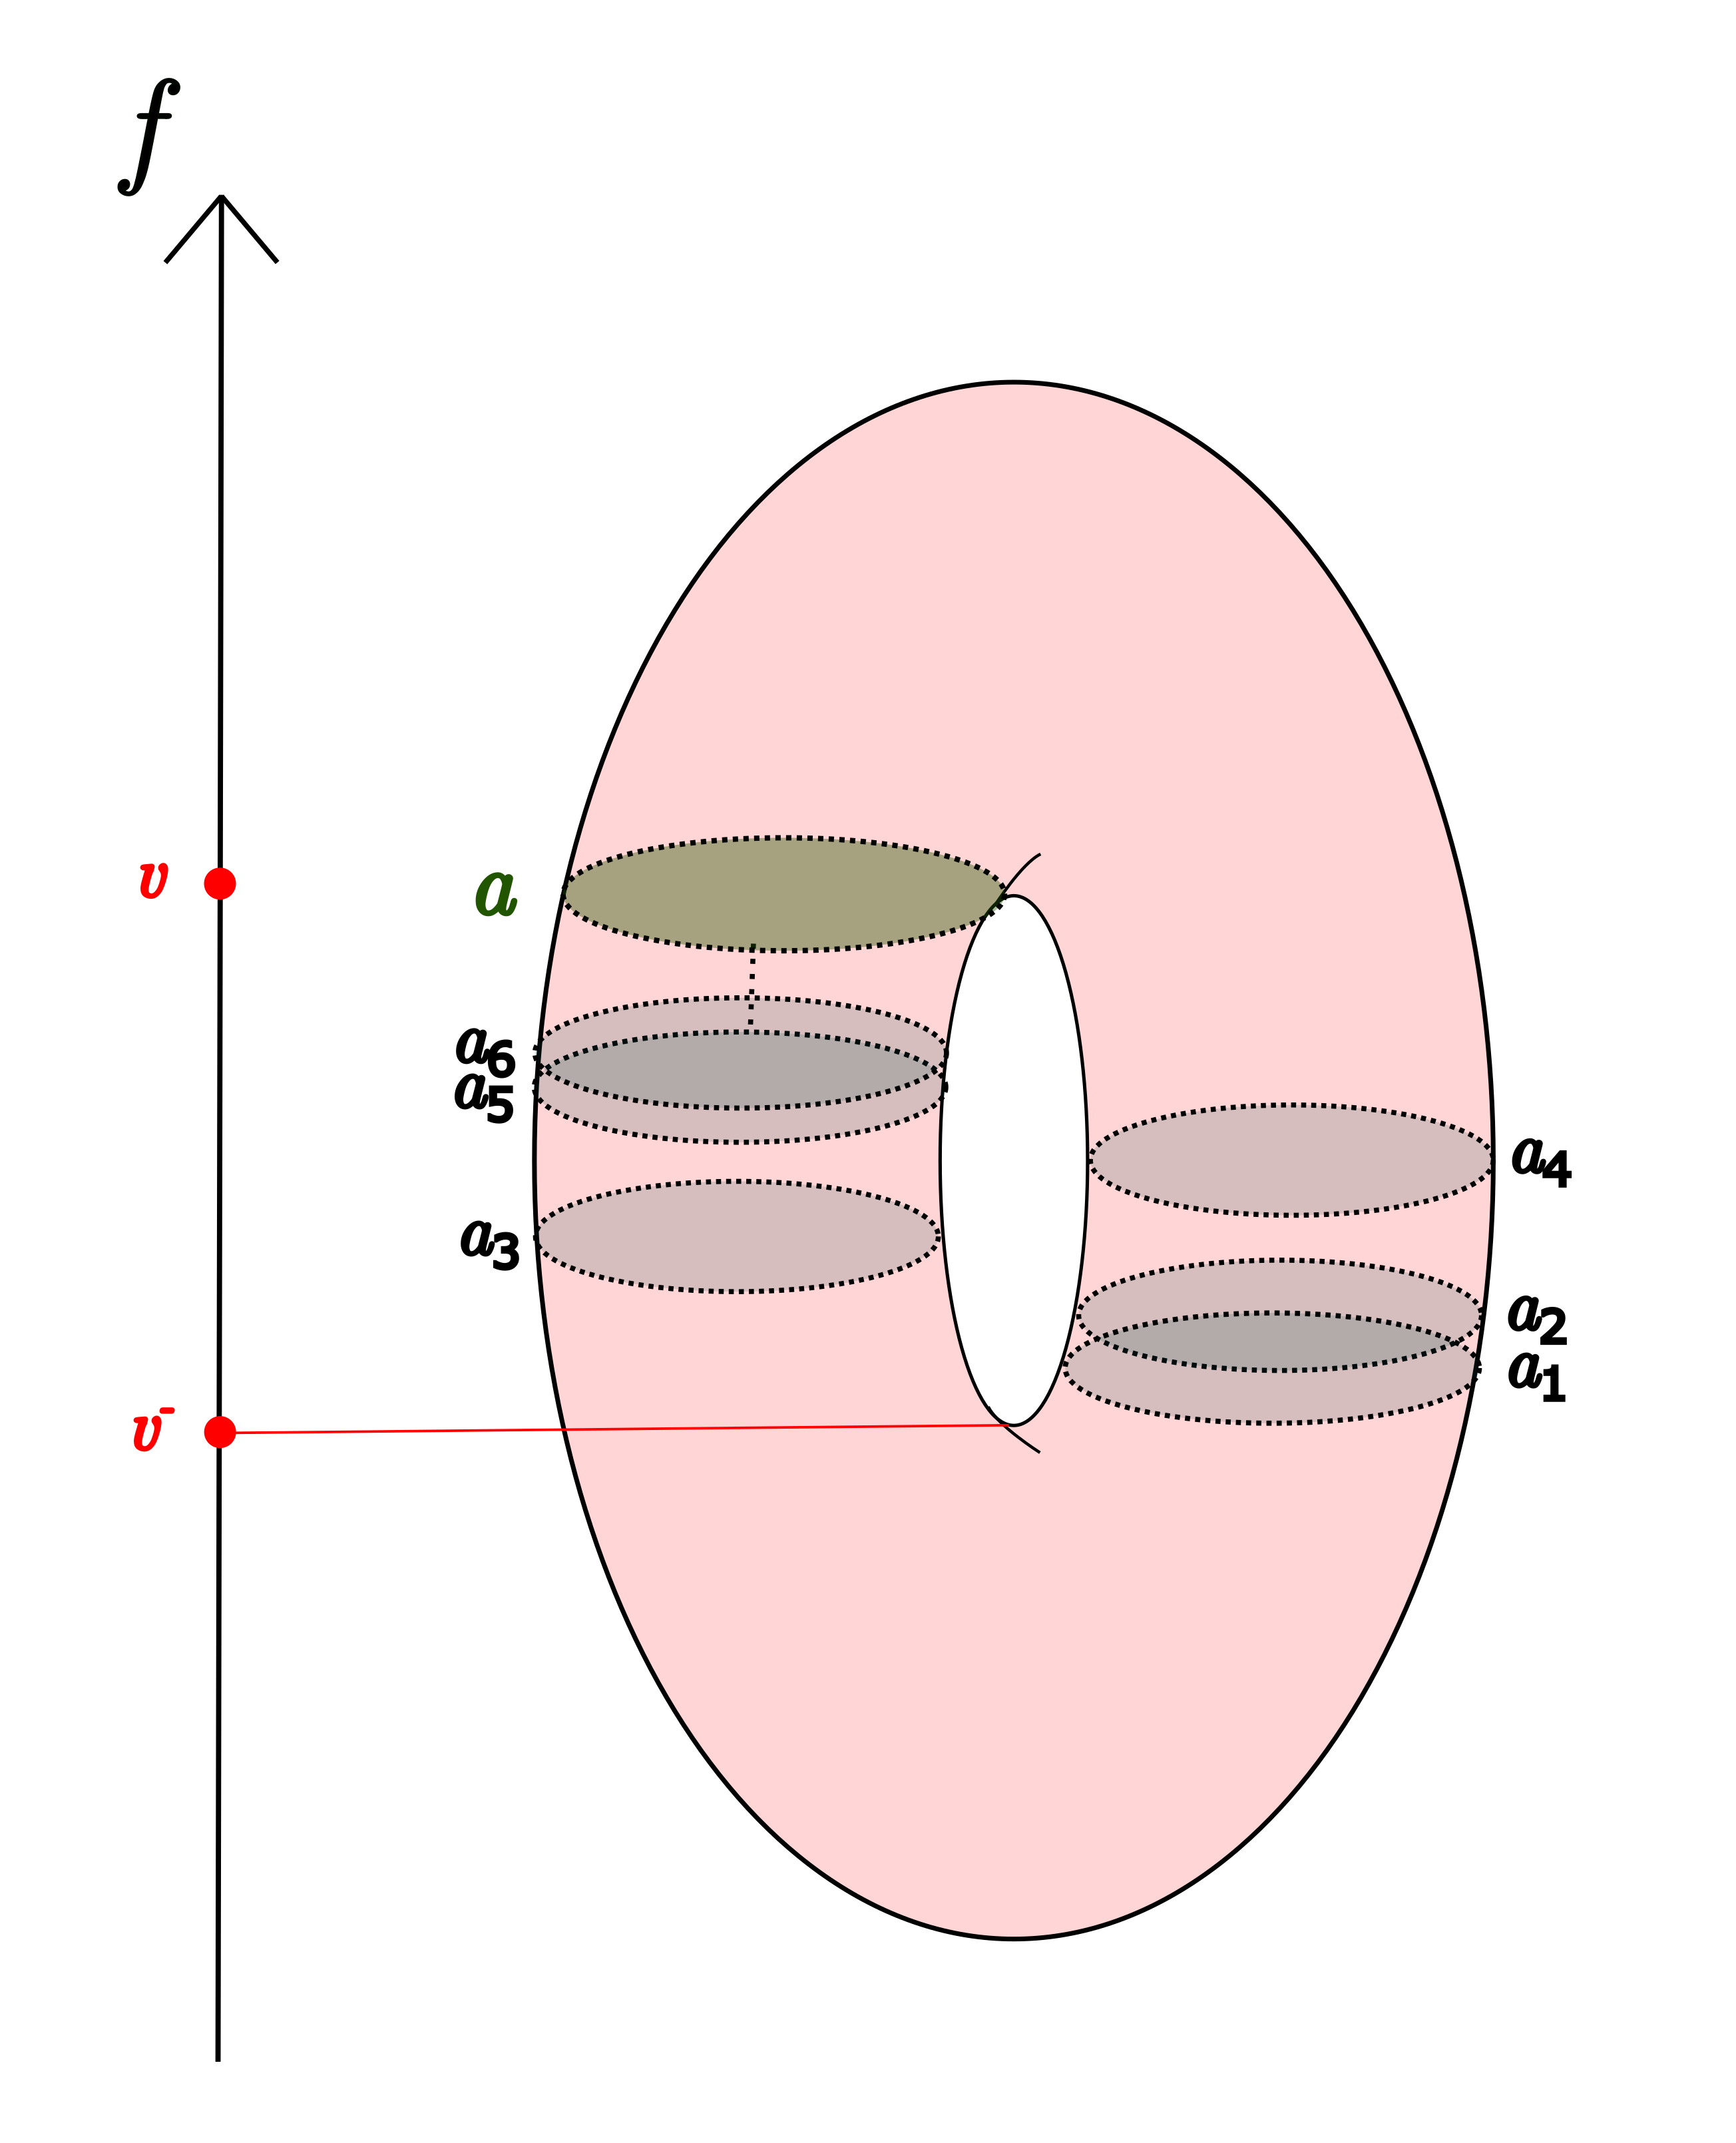
\includegraphics[width=0.4\textwidth]{images/reeb_tirroir.png}
    \caption{Example of a convergent sequence $(a_n)_{n\in\N}$ of Reeb graph elements  associated to filter values inside the open interval $(v^-,v)$. Since the number of cylinders in $\preim{f}{(v^-,v)}$ is finite, $(a_n)_{n\in\N}$ must have an infinite amount of terms inside one of them.}
    \label{fig:reeb_tirroir}
\end{figure}

\end{proof} 


We now consider a non-empty $a\in\overline{\reeb}\setminus\reeb$ and $v=\Tilde{f}(a)$ the corresponding critical value. By Lemma~\ref{lem:morse}, the set of critical values is finite because $\man$ is compact. It remains to check that the  preimage of a critical value is a finite set. 
 
Let $(a_n)_{n\in\N}$ be a sequence of elements in $\reeb$ that converges to $a$. If the first case of Lemma~\ref{lem:3cases} applies, then $(a_n)_{n\in\N}$ must be constant after a certain rank in order to converge because the number of connected components of $\preim{f}{\{v\}}$ is finite (see Proposition~\ref{prop:local_path_con}), which implies that $a\in\reeb$ leading to a contradiction because $a\in\overline{\reeb}\setminus\reeb$.


W.l.o.g. we assume that the second point of Lemma~\ref{lem:3cases} is satisfied for $a$. The following lemma allows to finish the proof of the proposition.

\begin{lemma}\label{lem:critical}
Let $a\in\overline{\reeb}$ such that $v=\Tilde{f}(a)$ is a critical value, and $v^-$ and  $v^+$ defined as in Lemma~\ref{lem:3cases}. Let $(u_n)_{n\in\N}$ and $(v_n)_{n\in\N}$ be two sequences in $[\frac{v^-+v}{2},v)$ such that $u_n\converge v$ and $v_n\converge v$. Let $c$ be a connected component of $\preim{f}{\{\frac{v^-+v}{2}\}}$. Then we have: 
$$\haus(\psi_{u_n-\frac{v^-+v}{2}}(c),\psi_{v_n-\frac{v^-+v}{2}}(c))\converge 0.$$
\end{lemma}

\begin{proof}
W.l.o.g., we assume that $u_n\leq v_n$. 
Let $\eps>0$. Denote $$\man_\eps=\man\setminus\bigcup_{c\in\critic(f)}\ball\left(c,\frac{\eps}{4\left|\critic(f)\right|}\right).$$ 
Since there are no critical values in $[u_n,v_n]$, we can use the gradient flow $(\psi_t)_t$ of $f$ (see Lemma~\ref{lem:flow}) to send any point $p$ in $\psi_{u_n-\frac{v^-+v}{2}}(c)$ to a point $q$ in $\psi_{v_n-\frac{v^-+v}{2}}(c)$ (and conversely) using the curve:
 \begin{align*}
 \gamma\colon[0,v_n-u_n]&\longrightarrow \man\\
 t&\longmapsto\psi_{t+u_n-\frac{v^-+v}{2}}(p),
 \end{align*}
where $\gamma(0)=p$ and $\gamma(v_n-u_n)=q$.\\
Now, for every $c\in\critic(f)$, if $\gamma$ enters $\ball\left(c,\frac{\eps}{4\left|\critic(f)\right|}\right)$, consider 
$$t^c_0=\inf\left\{t\in[0,v_n-u_n],\,\gamma(t)\in \ball\left(c,\frac{\eps}{4\left|\critic(f)\right|}\right)\right\},$$
and 
$$t^c_1=\sup\left\{t\in[0,v_n-u_n],\,\gamma(t)\in \ball\left(c,\frac{\eps}{4\left|\critic(f)\right|}\right)\right\}.$$
Otherwise, take $t^c_0=t^c_1=0$.
Notice that
$$\dis(\gamma(t^c_0),\gamma(t^c_1))\leq \frac{\eps}{2\left|\critic(f)\right|}.$$
 Denoting
 $$\mathcal{U}=[0,v_n-u_n]\setminus\bigcup_{c \in \critic(f)}[t^c_0,t^c_1],$$
 we have $\gamma\left(\mathcal{U}\right)\in\man_\eps$. We also  have:
\begin{align*}
\dis(p,q)&\leq\int_{t\in \mathcal{U}}\left\Vert\frac{d\psi_{t+u_n-\frac{v^-+v}{2}}(p)}{dt}\right\Vert\,dt + \sum_{c \in \critic(f)} \dis(\gamma(t^c_0),\gamma(t^c_1)) \\
&\leq\int_{t\in \mathcal{U}}\frac{dt}{\Vert\nabla f(\psi_{t+u_n-\frac{v^-+v}{2}}(p))\Vert} + \sum_{c \in \critic(f)} \frac{\eps}{2\left|\critic(f)\right|}\\
&\leq\frac{|v_n-u_n|}{\inf_{p\in\man_\eps}\Vert\nabla f(p)\Vert}+ \frac{\eps}{2}.
\end{align*}
Since $v_n-u_n\converge 0$ and $\inf_{p\in\man_\eps}\Vert\nabla f(p)\Vert > C$ for some $C>0$, for $n$ large enough we have $\dis(p,q)\leq\eps$, and finally $\haus(\psi_{u_n-\frac{v^-+v}{2}}(c),\psi_{v_n-\frac{v^-+v}{2}}(c))\converge 0$.

\end{proof}

 
Let $a\in\overline{\reeb}\setminus\reeb$ which satisfies the second case in Lemma~\ref{lem:3cases}, we thus have $a_{\phi(n)}=\psi_{v_n-\frac{v^-+v}{2}}(c)$ with $c$ being a connected component of $\preim{f}{\{\frac{v^-+v}{2}\}}$ and $v_n\converge v$.  According to Lemma ~\ref{lem:critical}, the limit of $(a_{\phi(n)})_{n\in\N}$ is the same as the limit of $(b_n)_{n\in\N}$ defined as:
$$\forall n\in\N:\,b_n=\begin{cases}
    c&\text{ if } v-\frac{1}{n}\leq\frac{v^-+v}{2},\\
    \psi_{v-\frac{1}{n}}(c)&\text{otherwise}.
\end{cases}$$
Finally, notice that $(b_n)_{n\in\N}$ depends only on $c$ and we showed that it converges to $a$. The number of connected components of $\preim{f}{\{\frac{v^-+v}{2}\}}$ and $\preim{f}{\{\frac{v^++v}{2}\}}$ being finite (see Proposition~\ref{prop:local_path_con}), the set $\left\{a\in\overline{\reeb},\,\Tilde{f}(a)=v\right\}$ is therefore also finite.\\\\
We conclude that $\overline{\reeb}\setminus\reeb$ is finite.
\end{proof}


\begin{proposition}\label{prop:reeb_sep}$(\overline{\reeb},\haus)$ is separable.
\end{proposition}


\begin{proof}
On one hand, $f$ is constant on the elements of $\overline{\reeb}$. As such, there is a map $\Tilde{f}_{|\reeb}$, that assigns to each element of $\reeb$ the unique value that $f$ takes on it. 
For each critical value $v$, $\preim{\Tilde{f}_{|\reeb}}{\{v\}}$ is finite. This is because $\preim{f}{\{v\}}$ is compact  and locally path-connected, and a locally path-connected compact space has finitely many connected components. 
Now, there are finitely many critical values of $f$ by Lemma~\ref{lem:morse}. Hence, denoting $C$ the union over all critical values $v$ of $\preim{\Tilde{f}_{|\reeb}}{\{v\}}$, one has that $C$ is finite. 

On the other hand, $\man$ is separable, and therefore there exists a countable subset $D$ of $\man$ such that $\man=\overline{D}$. We now show that the countable subset $E=C\cup \{[x]_{\sim_f},\,x\in D\}$ is dense in $\reeb$. Let $a\in\reeb$. 
\begin{itemize}
	\item If $\Tilde{f}_{|\reeb}(a)$ is a critical value, then $a\in C$.
	\item If $\Tilde{f}_{|\reeb}(a)$ is not a critical value, then let $x\in a$. Given that $x\in\man$ and $D$ is dense in $\man$, there exists $(x_n)_{n\in\N}$ in $D$ such that $x_n\converge x$. Consider the sequence $([x_n]_{\sim_f})_{n\in\N}$, by Lemma~\ref{lem:haus_cont} we have $[x_n]_{\sim_f}\converge a$.
\end{itemize}  

We showed that $E$ is dense in $\reeb$. Therefore, its closure in $\overline{\reeb}$ verifies $\reeb\subseteq\overline{E}$. Hence, $\overline{\reeb}=\overline{E}$.

\end{proof}

Consider the following map:
\begin{align*}
\pi\colon&\man\longrightarrow\overline{\reeb}\\
&x\longmapsto[x]_{\sim_f}.
\end{align*}
The image of $\pi$ is $\reeb$ and it consists of the composition of the natural map associated to the quotient of $\man$ by the equivalence relation $\sim_f$ with the inclusion of $\reeb$ in its closure.
 
 We introduce the notation $\mathcal{F}=\left\{x\in\man,\,f(x)\text{ is a critical value}\right\} $ for the set of points whose image under $f$ is a critical value.

\begin{proposition}\label{prop:pi_cont}  For every measure $\mes$ on $(\man,\dis)$ such that $\mes(\mathcal{F})=0$, one has that
$\pi$ is continuous $\mes$-almost everywhere.
\end{proposition}

\begin{proof}
We will prove that the map $\pi$ is continuous at every point $x\in\man$ such that $f(x)$ is not a critical value. Let $x$ be such a point and let $(x_n)_{n\in\N}$ be a sequence in $\man$ such that $x_n\converge x$. By Lemma~\ref{lem:haus_cont}, one has $$\pi(x_n)=[x_n]_{\sim_f}\converge \pi(x)=[x]_{\sim_f}.$$
\end{proof}


\begin{lemma}\label{lem:zero_measure}
If a measure $\mes$ is absolutely continuous with respect to the volume measure, then $\mes(\mathcal{F})=0$.
\end{lemma}
\begin{proof}
The set $\critic(f)$ is finite and hence closed. As such, $\man'=\man\setminus\critic(f)$ is an open submanifold of $\man$. Now,
$$\mathcal{F}=\critic(f)\cup \left[\mathcal{F}\cap \man'\right],$$
and by the Implicit Function Theorem (see Theorem 5.8. of~\cite{boothby1986introduction} for example), $\mathcal{F}\cap \man'$ is a finite union of $(d-1)-$dimensional submanifolds in $\man$ as the critical values of $f$ in $\man$ are no longer critical in $\man'$. Hence
$$\mes\left( \mathcal{F}\cap \man'\right)=0.$$
Finally, $\mes(\mathcal{F})=0$.
%Recall that $\mathcal{F}=\left\{x\in\man,\,f(x)\text{ is critical}\right\}$.\\ $\man$ is a compact manifold, therefore it admits a finite atlas $(U_i)_{1\leq i\leq I}$.\\
%Furthermore, $$\mathcal{F}=\critic(f)\cup \bigcup_{\substack{1\leq i\leq I \\k\in\mathbb{N}}} \mathcal{F}\cap U_i\setminus\left(\bigcup_{c\in\critic(f)}\ball(c,1/k)\right).$$\\
%Now, $f$ has no critical points on each $V_{i,k}=U_i\setminus\left(\bigcup_{c\in\critic(f)}\ball(c,1/k)\right)$, which admits a manifold structure because it is homeomorphic to an open set in a Euclidean space.\\ By the implicit function theorem (see Theorem 5.8. of~\cite{boothby1986introduction} for example), $\mathcal{F}\cap V_{i,k}$ is a lower-dimensional submanifold and has therefore zero measure.\\
%$\critic(f)$ is finite by Lemma~\ref{lem:morse} and as such also has zero measure.\\
%Finally, $\mathcal{F}$ is a countable union of zero measure sets, hence, $\mu(\mathcal{F})=0$.
\end{proof}


\begin{corollary}\label{cor:pi_mes}
$\pi$ is Borel measurable.
\end{corollary}

Following Proposition~\ref{prop:reeb_sep} and Corollary~\ref{cor:pi_mes}, we can now consider the metric measure space $(\overline{\reeb},\haus,\vol\circ\pi^{-1})$. Notice that since the image of $\pi$ is $\reeb$, $\vol\circ\pi^{-1}(\reeb)=\vol(\man)$.

